\documentclass[../lecture-notes.tex]{subfiles}

\begin{document}

\subsection{What is zk-SNARK?}

\subsubsection{Informal Overview}

Finally, we've reached the most interesting part of the course, where we will consider various zk-SNARK constructions we are using on the daily basis. Again, recall that we have the presence of two parties:
\begin{itemize}
    \item \textbf{Prover} $\mathcal{P}$ --- the party who knows the data that can resolve the given problem.
    \item \textbf{Verifier} $\mathcal{V}$ --- the party that wants to verify the given proof.
\end{itemize}

Here, the prover wants to convince the verifier that they know the data that resolves the problem (typically, some complex computation) without revealing the data (witness) itself. In the previous lecture, we defined the first practical primitive: zk-NARK --- a \textit{zero-knowledge non-interactive argument of knowledge}, and gave the first widely used example: non-interactive Schnorr protocol (which is a special case of a $\Sigma$-protocol with the Fiat-Shamir transformation applied). Now, we add one more component which completely changes the game and significantly extends the number of applications: \textbf{succinctness}.

\begin{definition}
    \textbf{zk-SNARK} --- Zero-Knowledge \textbf{Succinct} Non-interactive ARgument of Knowledge.
\end{definition}

Again, since this is a central question considered, we need to recall what do terms like ``argument of knowledge``, ``succinct``, ``non-interactive``, and 
``zero-knowledge`` mean in this context:

\begin{itemize}
    \item \textbf{Argument of Knowledge} --- a proof that the prover knows the data (witness) that resolves a certain
    problem, and this knowledge can be ``extracted''.
    \item \textbf{Succinctness} --- the proof size and verification time is relatively small relative to the computation size and sometimes even does not depend on the size of 
    the data or statement. This will be explained with examples later.
    \item \textbf{Non-interactiveness} --- to produce the proof, the prover does not need any interaction
    with the verifier.
    \item \textbf{Zero-Knowledge} --- the verifier learns nothing about the data used to produce the
    proof, despite knowing that this data resolves the given problem and that the prover possesses it.
\end{itemize}

In essence, zk-SNARKs allow one party to prove to another that they know a value without revealing 
any information about the value itself, and do so with a proof that is both very small and quick to 
verify. This makes zk-SNARKs a powerful tool for maintaining privacy and efficiency in various 
cryptographic applications.

This is pretty wide defined and maybe not so obvious if you do not have any background. Let us take a
look at the example.

\begin{example}
    Imagine you are the part of a treasure hunt, and you've found a hidden treasure chest. You want to 
    prove to the treasure hunt organizer that you know where the chest is hidden without revealing
    its location. Here's how zk-SNARKs can be used in this context: \\

    \textbf{The problem}: you have found a hidden treasure chest (the secret data), and you want to
    prove to the organizer (the verifier) that you know its location without actually revealing 
    where it is. \\

    \textbf{How zk-SNARKs Help}:

    \begin{itemize}
        \item \textbf{Argument of Knowledge}: You create a proof that demonstrates you know the exact
        location of the treasure chest. This proof convinces the organizer that you have this 
        knowledge.
        \item \textbf{Succinctness}: The proof you provide is very small and concise. It doesn't matter how
        large the treasure map is or how many steps it took you to find the chest, the proof remains
        compact and easy to check.
        \item \textbf{Non-interactiveness}: You don't need to have a back-and-forth conversation with the 
        organizer to create this proof. You prepare it once. The organizer can verify it without 
        needing to ask you any questions.
        \item \textbf{Zero-Knowledge}: The proof doesn't reveal any information about the actual location of
        the treasure chest. The organizer knows you found it, but they don't learn anything about 
        where it is hidden. \\
    \end{itemize}

    Here you can think of zk-SNARK as a golden coin from the chest where the pirates' sign is 
    engraved, so the organizer can be sure you've found the treasure.
\end{example}

But the problems that we want to solve are in a slightly different format. We can't bring a coin to
the verifier. Our goal is to prove that we've executed a specific program on a set of data that 
resolves a specific challenge or gives us a particular result.

\subsubsection{Formal Definition}

In this section, we will provide a more formal definition of zk-SNARKs. In case you do not want to
dive into the technical details, you can skip this part and move to the next sections where we will
consider the arithmetic circuits and the Quadratic Arithmetic Programs.

Previously, we considered NARKs that did not require any setup procedure. However, zk-SNARKs are
more complex and require a setup phase. This setup phase is used to generate the proving and
verification keys (which we call prover parameters $\mathsf{pp}$ and verifier parameters $\mathsf{vp}$, respectively), 
which are then used to create and verify proofs. That being said, let us introduce the \textbf{preprocessing NARK}.

\begin{definition}
    A \textbf{preprocessing non-interactive argument of knowledge} (\textbf{preprocessing NARK}) $\Pi_{\text{preNARK}}=(\mathsf{Setup},\mathsf{Prove},\mathsf{Verify})$ consists of three algorithms:
    \begin{itemize}
        \item $\mathsf{Setup}(1^\lambda) \rightarrow (\mathsf{pp}, \mathsf{vp})$ --- the setup algorithm that takes the security parameter $\lambda$ and outputs the public parameters: proving and verification keys.
        \item $\mathsf{Prove}(\mathsf{pp}, x, w) \rightarrow \pi$ --- the proving algorithm that takes the prover parameters $\mathsf{pp}$, statement $x$, and witness $w$, and outputs a proof $\pi$.
        \item $\mathsf{Verify}(\mathsf{vp}, x, \pi) \rightarrow \{\mathsf{accept}, \mathsf{reject}\}$ --- the verification algorithm that takes the verification key, statement $x$, and proof $\pi$, and outputs a bit indicating whether the proof is valid.
    \end{itemize}
\end{definition}

Recall, that from NARK (and now preprocessing NARK, respectively) over relation $\mathcal{R}$ we require the following properties:
\begin{itemize}
    \item \textbf{Completeness} --- if the prover is honest and the statement is true, the verifier will always accept the proof:
    \begin{equation*}
        \forall (x,w) \in \mathcal{R}: \text{Pr}[\mathsf{Verify}(\mathsf{vp}, x, \mathsf{Prove}(\mathsf{pp},x,w)) = \mathsf{accept}] = 1
    \end{equation*}
    \item \textbf{Knowledge Soundness} --- the prover cannot (statistically) generate a false proof $\pi$ that convinces the verifier. 
    \item \textbf{Zero-knowledge} --- the verifier ``learns nothing'' about the witness $w$ from $(\mathcal{R},\mathsf{pp},\mathsf{vp},x,\pi)$.
\end{itemize}

While we have formally defined all the terms here, including statistical soundness, we have not defined what \textbf{knowledge soundness} is. We give a brief informal definition below.

\begin{definition}[Knowledge Soundness]
    $\Pi_{\text{preNARK}}$ is (adaptively) \textbf{knowledge sound} for a relation $\mathcal{R}$ if for every PPT adversary $\mathcal{A}=(\mathcal{A}_0,\mathcal{A}_1)$, split into two algorithms, such that:
    \begin{equation*}
        \text{Pr}\begin{bmatrix}[c|c]
            & (\mathsf{pp},\mathsf{vp}) \gets \mathsf{Setup}(\cdot)\\
            \mathsf{Verify}(\mathsf{vp},x,\pi)=\mathsf{accept} & x \gets \mathcal{A}_0(\cdot)  \\
            & \pi \gets \mathcal{A}_1(\mathsf{pp},x)
        \end{bmatrix} > \alpha,
    \end{equation*}
    where $\alpha=\alpha(\lambda) \neq \mathsf{negl}(\lambda)$ is a non-negligible probability, there exists a PPT extractor $\mathcal{E}^{\mathcal{A}}$ such that
    \begin{equation*}
        \text{Pr}\begin{bmatrix}[c|c]
            (x,w) \in \mathcal{R} & x \gets \mathcal{A}_0(\cdot), \; w \gets \mathcal{E}^{\mathcal{A}}(x)
        \end{bmatrix} > \alpha - \epsilon,
    \end{equation*}
    where $\epsilon = \epsilon(\lambda)$ is a negligible function.
\end{definition}

\begin{remark}
    Informally, the aforementioned definition means that if the prover can generate a false proof with a non-negligible probability, then there exists an extractor that can extract the witness with a probability that is almost as high (and thus is also non-negligible).
\end{remark}

Finally, to make zk-NARKs more universal and applicable to a wider range of problems, we introduce the \textbf{zk-SNARK} by adding the \textbf{succinctness} property.

\begin{definition}
    A \textbf{zk-SNARK} (Succint NARK) is a preprocessing NARK, where the proof's length $|\pi|$ and verification time $T_{\mathcal{V}}$ are short: the verification time is sublinear in the size of the computation $C$ (denoted by $|C|$), while the proof size is sublinear in the witness size $|w|$:
    \begin{equation*}
        |\pi| = \mathsf{sublinear}(|w|), \; T_{\mathcal{V}} = O_{\lambda}(|x|, \mathsf{sublinear}(|C|)).
    \end{equation*}
\end{definition}

\begin{remark}
    \textbf{Sublinearity} means that the function $f: \mathbb{N} \to \mathbb{R}$ grows slower than linearly. For example, functions $f(n) = \log n$ or $f(n) = \sqrt{n}$ are sublinear, while $f(n) = 3n+2$ is linear. Generally, if $f(n)/(c\cdot n) \xrightarrow[n \to \infty]{} 0$ for any $c \in \mathbb{R}\setminus \{0\}$, then $f(n)$ is sublinear.
\end{remark}

\begin{example}
    Consider the protocol where the proof size is $|\pi| = O(\sqrt{|w|})$ and $T_{\mathcal{V}} = O(\sqrt[3]{|C|})$. Such protocol is a zk-SNARK, as the proof size is sublinear in the witness size and the verification time is sublinear in the size of the computation.
\end{example}

Although having a proof size and verification time lower than linear is nice, that is still not sufficient to make zk-SNARKs practical in the wild. For that reason, typically, in practice, we require a stricter definition of the succinctness property, where the proof size and verification time are constant or logarithmic in the size of the computation. This is the case for most zk-SNARKs used in practice.
\begin{definition}
    A \textbf{zk-SNARK} is \textbf{strongly succinct} if the proof size and verification time are constant or logarithmic in the size of the computation:
    \begin{equation*}
        |\pi| = O_{\lambda}(\log |C|), \; T_{\mathcal{V}} = O_{\lambda}(|x|, \log|C|).
    \end{equation*}
\end{definition}

\begin{example}
    Consider three major proving systems used in practice with $N=|C|$ being the complexity of a computation:
    \begin{itemize}
        \item \textbf{Groth16} with $|\pi| = O_{\lambda}(1)$, $T_{\mathcal{V}} = O_{\lambda}(1)$ is definitely a strongly succinct zk-SNARK since both the proof size and verification time are constant.
        \item \textbf{STARK}s with $|\pi| = O_{\lambda}(\mathsf{polylog}(N))$ and $T_{\mathcal{V}} = O_{\lambda}(\mathsf{polylog}(N))$ are also strongly succinct zk-SNARKs since both the proof size and verification time are logarithmic in the size of the computation.
        \item \textbf{Bulletproofs} with $|\pi| = O_{\lambda}(\log N)$ and $T_{\mathcal{V}} = O_{\lambda}(N)$ is not a strongly succinct zk-SNARK since the verification time is linear in the size of the computation.
    \end{itemize}
\end{example}

\subsection{Arithmetic Circuits}

\subsubsection{What is Arithmetic Circuit?}
The cryptographic tools we have learned in the previous lectures operate with numbers or certain 
primitives above them (like finite field extensions or elliptic curves), so the first question is: how do we convert a program into a mathematical 
language? Additionally, we need to do this in a way that can be further (a) made succinct, (b) allows us to prove 
something about it, and (c) be as universal as possible (to be able to prove quite general statements unlike $\Sigma$-protocols considered in the previous lecture).

The \textbf{Arithmetic Circuits} can help us with these problems. Similar to \textbf{Boolean Circuits}, they consist of \textbf{gates} and 
\textbf{wires}: gates represent operations acting all elements, connected by wires (see figure below for details). Yet, instead of operations $\mathtt{AND}$, $\mathtt{OR}$, $\mathtt{NOT}$ and such, in arithmetic circuits only 
multiplication/addition/subtraction operations are allowed. Additionally, arithmetic circuits manipulate over elements
from some finite field $\mathbb{F}$ (see right figure below).

% --- Writing diagrams ---

% Define circle styles and colors
\colorlet{circle edge}{gray!50!black}
\colorlet{circle area}{gray!20}
\colorlet{gate1 edge}{green!50!black}
\colorlet{gate1 area}{green!20}
\colorlet{gate2 edge}{orange!50!black}
\colorlet{gate2 area}{orange!20}
\colorlet{gate3 edge}{blue!50!black}
\colorlet{gate3 area}{blue!20}

\tikzset{
    var/.style={circle, draw=circle edge, fill=circle area, very thick, minimum size=1cm, text centered},
    gate1/.style={circle, draw=gate1 edge, fill=gate1 area, ultra thick, minimum size=1cm, text centered},
    gate2/.style={circle, draw=gate2 edge, fill=gate2 area, ultra thick, minimum size=1cm, text centered},
    gate3/.style={circle, draw=gate3 edge, fill=gate3 area, ultra thick, minimum size=1cm, text centered},
    arrow/.style={-Stealth, ultra thick}
}

\begin{figure}[h!]
    \centering
    \vspace*{1em}
    
    \begin{minipage}{0.46\textwidth}
        \centering
        % Boolean AND and OR gates
        \begin{tabular}{cc}
            \begin{tikzpicture}
                % Nodes
                \node[var] (a) at (0, -1.5) {$a$};
                \node[var] (b) at (2, -1.5) {$b$};
                \node[gate1] (and) at (1, 0) {\texttt{AND}};
                \node[var] (c) at (1, 1.75) {$c$};

                % Arrows
                \draw[arrow,gray] (a) -- (and);
                \draw[arrow,gray] (b) -- (and);
                \draw[arrow,gray!50!black] (and) -- (c);
            \end{tikzpicture}
            &
            \begin{tikzpicture}
                % Nodes
                \node[var] (a) at (0, -1.5) {$a$};
                \node[var] (b) at (2, -1.5) {$b$};
                \node[gate2] (or) at (1, 0) {\texttt{OR}};
                \node[var] (c) at (1, 1.75) {$c$};

                % Arrows
                \draw[arrow,gray] (a) -- (or);
                \draw[arrow,gray] (b) -- (or);
                \draw[arrow,gray!50!black] (or) -- (c);
            \end{tikzpicture}
            \label{fig:circuits}
        \end{tabular}
        \caption{Boolean \texttt{AND} and \texttt{OR} Gates}
    \end{minipage}
    \hspace{0.05\textwidth} % Space between figures
    \begin{minipage}{0.46\textwidth}
        \centering
        % Addition and Multiplication gates
        \begin{tabular}{cc}
            \begin{tikzpicture}
                % Nodes
                \node[var] (a) at (0, -1.5) {$a$};
                \node[var] (b) at (2, -1.5) {$b$};
                \node[gate1] (add) at (1, 0) {$+$};
                \node[var] (c) at (1, 1.75) {$c$};

                % Arrows
                \draw[arrow,gray] (a) -- (add);
                \draw[arrow,gray] (b) -- (add);
                \draw[arrow,gray!50!black] (add) -- (c);
            \end{tikzpicture}
            &
            \begin{tikzpicture}
                % Nodes
                \node[var] (a) at (0, -1.5) {$a$};
                \node[var] (b) at (2, -1.5) {$b$};
                \node[gate2] (mul) at (1, 0) {$\times$};
                \node[var] (c) at (1, 1.75) {$c$};

                % Arrows
                \draw[arrow,gray] (a) -- (mul);
                \draw[arrow,gray] (b) -- (mul);
                \draw[arrow,gray!50!black] (mul) -- (c);
            \end{tikzpicture}
        \end{tabular}
        \caption{Addition and Multiplication Gates}
    \end{minipage}
    \vspace*{1em}
\end{figure}

\begin{wraptable}{r}{0.4\textwidth}
    \centering
    \vspace{-1em}
    \begin{tabular}{|c|c|c|}
        \hline
        \textbf{A} & \textbf{B} & \textbf{A AND B} \\
        \hline
        0 & 0 & 0 \\
        \hline
        0 & 1 & 0 \\
        \hline
        1 & 0 & 0 \\
        \hline
        1 & 1 & 1 \\
        \hline
    \end{tabular}
    \caption{\texttt{AND} Gate Truth Table}
    \label{tab:and-truth-table}
    \vspace{1em}
\end{wraptable}

% --- Finish Writing diagrams ---

Let us come back to boolean circuits for a moment and consider the \texttt{AND} gate. The \textit{\texttt{AND} Gate Truth \Cref{tab:and-truth-table}} shows us the results we receive if 
particular values are supplied to the gate. The main point here is that with this table, we can 
verify the validity of logical statements. Boolean circuits receive an input vector of $\{0, 1\}$ 
and resolve to \texttt{true} (1) or \texttt{false} (0); basically, they determine if the input values satisfy the 
statement.

However, more notably, we can combine these gates to create more complex circuits that can resolve
more complex problems. For example, we might construct a circuit depicted in \Cref{fig:bool-circuit}, 
calculating $(a \;\texttt{AND}\; b) \,\texttt{OR}\; c$.

\begin{figure}[h!]
    \centering
    \begin{tikzpicture}
        % Nodes
        \node[var] (a) at (0, -1.5) {$a$};
        \node[var] (b) at (2, -1.5) {$b$};
        \node[var] (c) at (4, -1.5) {$c$};
        \node[gate1] (and) at (1, 0) {\texttt{AND}};
        \node[gate2] (or) at (3, 1.5) {\texttt{OR}};
        \node[var] (d) at (5, 1.5) {$d$};

        % Arrows
        \draw[arrow,gray] (a) -- (and);
        \draw[arrow,gray] (b) -- (and);
        \draw[arrow,gray] (c) -- (or);
        \draw[arrow,gray] (and) -- (or);
        \draw[arrow,gray!50!black] (or) -- (d);
    \end{tikzpicture}
    \caption{Example of a circuit evaluating $d = (a \;\texttt{AND}\; b) \,\texttt{OR}\; c$.}
    \label{fig:bool-circuit}
\end{figure}

Although we can already represent very complex computations using boolean circuits\footnote{\ldots such as \texttt{SHA-256} hash function computation, one might take a look here: \url{http://stevengoldfeder.com/projects/circuits/sha2circuit.html}}, they are not the most convenient way to represent arithmetic operations. 

That being said, we can do the same with \textbf{arithmetic circuits} to verify computations over some finite field $\mathbb{F}$ without excessive 
verbosity due to a binary arithmetic, where we had to perceive all intermediate
values as binary $\{0,1\}$.

\subsubsection{More advanced examples}

Let us take a look at some examples of programs and how can we translate them to the arithmetic
circuits. 

\textbf{Example 1: Multiplication.} Consider a very simple program, where we are to simply multiply two field elements $a,b \in \mathbb{F}$:

\begin{lstlisting}[language=Python,numbers=none]
    def multiply(a: F, b: F) -> F:
        return a * b
\end{lstlisting}

Since we are doing all the arithmetic in a finite field $\mathbb{F}$, we denote it by \texttt{F} in the code. This can be represented as a circuit with only one (multiplication) gate:
\begin{equation*}
    r = a \times b
\end{equation*}    

The witness vector (essentially, our solution vector) is $\mathbf{w} = (r, a, b)$, for example: $(6, 2, 3)$. We 
assume that the $a$ and $b$ are input values. 

We can think of the ``=`` in the gate as an assertion, meaning that if $a \times b$ does not equal
$r$, the assertion fails, and the input values do not resolve the circuit.

Good, but this one is quite trivial. Let's consider a more complex example.

\textbf{Example 2: Multivariate Polynomial.} Now, suppose we want to implement the evaluation of the polynomial $Q(x_1,x_2) = x_1^3 + x_2^2 \in \mathbb{F}[X_1,X_2]$ using arithmetic circuits. The corresponding program is as follows:
\begin{lstlisting}[language=Python,numbers=none]
    def evaluate(x1: F, x2: F) -> F:
        return x1**3 + x2**2
\end{lstlisting}

Looks easy, right? But the circuit is now much less trivial. Consider \Cref{fig:multivariate-polynomial-circuit}. Notice that to calculate $x_1^3$ we cannot use the single gate: we need to multiply $x_1$ by itself two times. For that reason, we need three multiplication and one addition gate to represent $Q(x_1,x_2)$ calculation.
\begin{figure}[h!]
    \centering
    \begin{tikzpicture}
        % Nodes
        \node[var] (x1) at (0, 1) {$x_1$};
        \node[gate2] (x1_x1) at (2, 1) {$\times$};
        \node[gate2] (x1_x1_x1) at (4, 1) {$\times$};

        \node[var] (x2) at (0, -1) {$x_2$};
        \node[gate2] (x2_x2) at (2, -1) {$\times$};

        \node[gate1] (plus) at (5.0, -0.5) {$+$};

        % x1**3
        \draw[arrow,gray] (x1) to [bend left=45] (x1_x1);
        \draw[arrow,gray] (x1) to [bend right=15] (x1_x1);
        \draw[arrow,gray] (x1_x1) -- (x1_x1_x1);
        \draw[arrow,gray] (x1) to [bend right=45] (x1_x1_x1);

        % x2**2
        \draw[arrow,gray] (x2) to [bend left=30] (x2_x2);
        \draw[arrow,gray] (x2) to [bend right=30] (x2_x2);

        % Summation
        \draw[arrow,gray] (x1_x1_x1) -- (plus);
        \draw[arrow,gray] (x2_x2) -- (plus);

        % Result
        \node[var] (q) at (7.0, -0.5) {$Q$};
        \draw[arrow,gray!50!black] (plus) -- (q);
    \end{tikzpicture}
    \caption{Example of a circuit evaluating $x_1^3 + x_2^2$.}
    \label{fig:multivariate-polynomial-circuit}
\end{figure}


\textbf{Example 3. \texttt{if} statements.} Well, it is quite clear how to represent any polynomial-like expressions. But how can we translate \texttt{if} statements? Consider the program below:

\begin{lstlisting}[language=Python,numbers=none]
    def if_statement_example(a: bool, b: F, c: F) -> F:
        return b * c if a else b + c
\end{lstlisting}

We can express this logic in mathematical terms as follows: ``If $a$ is true, compute 
$b \times c$; otherwise, compute $b + c$.'' However, only numerical expressions are allowed, so how can we proceed? Assuming that
$\texttt{true}$ is represented by $1$ and $\texttt{false}$ by $0$, we can transform this logic as follows:
\begin{equation*}
    r = a \times (b \times c) + (1 - a) \times (b + c)    
\end{equation*}

Now, what is the witness vector in this case? One might assume that $\mathbf{w} = (r, a, b, c)$ would suffice. Then, examples of valid witnesses include $(6, 1, 2, 3)$, $(5, 0, 2, 3)$.

But, we need to verify all the intermediate steps! This can be achieved by transforming the above
equation using the simplest terms (the gates), ensuring the correctness of each step in the program.

Below, we show to visualize the arithmetic circuit for the \texttt{if} statement example.

\begin{figure}[h!]
    \centering
    \begin{tikzpicture}
        % Nodes
        \node[var] (c) at (0, -3) {$c$};
        \node[var] (b) at (0, -1.5) {$b$};
        \node[var] (a) at (0, 0) {$a$};
        \node[var] (one) at (0, 1.5) {$1$};

        % b+c and b*c gates
        \node[gate1] (b_plus_c) at (3, -1.5) {$+$};
        \node[gate2] (b_times_c) at (3, -3.0) {$\times$};

        \node[gate3] (one_minus_a) at (3, 0.75) {$-$};

        % a*b*c and (1-a)(b+c) gates
        \node[gate2] (a_times_b_times_c) at (6, -2.0) {$\times$};
        \node[gate2] (one_minus_a_times_b_plus_c) at (6, -0.5) {$\times$};

        % a*b*c + (1-a)(b+c) gate
        \node[gate1] (r) at (9, -1.25) {$+$};

        % Result node
        \node[var] (result) at (11.5, -1.25) {$r$};

        % b+c and b*c arrows
        \draw[arrow,gray] (b) to (b_plus_c);
        \draw[arrow,gray] (b) to (b_times_c);
        \draw[arrow,gray] (c) to (b_plus_c);
        \draw[arrow,gray] (c) to (b_times_c);

        % 1 - c arrow
        \draw[arrow,gray] (one) to (one_minus_a);
        \draw[arrow,gray] (a) to (one_minus_a);

        % a*b*c and (1-a)(b+c) arrows
        \draw[arrow,gray] (a) to [bend left=20] (a_times_b_times_c);
        \draw[arrow,gray] (b_times_c) to node[midway, above] {$r_1$} (a_times_b_times_c);
        \draw[arrow,gray] (one_minus_a) to node[midway, above] {$r_3$} (one_minus_a_times_b_plus_c);
        \draw[arrow,gray] (b_plus_c) to node[midway, above] {$r_2$} (one_minus_a_times_b_plus_c);

        % a*b*c + (1-a)(b+c) arrows
        \draw[arrow,gray] (a_times_b_times_c) to [bend right=20] node[midway, above] {$r_4$} (r);
        \draw[arrow,gray] (one_minus_a_times_b_plus_c) to [bend left=20] node[midway, above] {$r_5$} (r);

        % Result arrow
        \draw[arrow,gray!50!black] (r) to (result);

    \end{tikzpicture}
    \caption{Example of a circuit evaluating the \texttt{if} statement logic.}
    \label{fig:multivariate-polynomial-circuit}
\end{figure}

Corresponding equations for the circuit are:

\begin{equation*}
    \begin{aligned}
        r_1 = b \times c \hspace{10px} & & &
        r_2 = b + c \\
        r_3 = 1 - a \hspace{10px} & & &
        r_4 = a \times r_1 \\
        r_5 = r_3 \times r_2 \hspace{10px} & & &
        r = r_4 + r_5 \\
    \end{aligned}
\end{equation*}

With the witness vector: $\mathbf{w} = (r, r_1, r_2, r_3, r_4, r_5, a , b, c)$. One example of a valid witness is $(6, 6, 5, 0, 6, 0, 1, 2, 3)$.

\subsubsection{Circuit Satisfability Problem}

Now, let us generalize what we have constructed so far. First, we begin with the arithmetic circuit.

\newcommand{\Circ}{\textit{\texttt{C}}}
\begin{definition}
    Arithmetic circuit $\Circ: \mathbb{F}^n \to \mathbb{F}$ with $n$ inputs over a finite field $\mathbb{F}$ is a directed acyclic graph where internal nodes are labeled via $+$, $-$, and $\times$, and inputs are labeled $1,x_1,x_2,\dots,x_n$. By $|\Circ|$ we denote the number of gates in the circuit.
\end{definition}

\begin{example}
    For example, previously considered multivariate polynomial $\Circ(x_1,x_2) = x_1^3 + x_2^2$ can be represented as an arithmetic circuit with three multiplication and one addition gates, as shown in \Cref{fig:multivariate-polynomial-circuit}. It is defined over inputs $\mathbf{x}=(x_1,x_2)$ with $n=2$ and $|\Circ| = 4$.
\end{example}

Now, suppose that the circuit is defined over $n$ inputs. We can always split this input into two parts: the first $\ell$ inputs are the \textit{public inputs}, being our statement $\mathbf{x} \in \mathbb{F}^{\ell}$, and the remaining $n-\ell$ inputs are the \textit{private inputs}, being our secret witness $\mathbf{w} \in \mathbb{F}^{n-\ell}$. The public inputs are known to everyone, while the private inputs are known only to the prover. The goal of the prover is to show that the circuit is satisfiable, i.e., that for the given $\mathbf{x}$, he \textit{knows} a witness $\mathbf{w}$ that resolves the circuit. Resolving in this context means that the output of the circuit is zero.

\begin{definition}
    The \textbf{Circuit Satisfiability Problem} is defined as follows: given an arithmetic circuit $\Circ$ and a public input $\mathbf{x} \in \mathbb{F}^{\ell}$, determine if there exists a private input $\mathbf{w} \in \mathbb{F}^{n-\ell}$ such that $\Circ(\mathbf{x},\mathbf{w}) = 0$. More formally, the problem is determined by relation $\mathcal{R}_{\Circ}$ and corresponding language $\mathcal{L}_{\Circ}$ as follows:
    \begin{equation*}
        \mathcal{R}_{\Circ} = \{(\mathbf{x},\mathbf{w}) \in \mathbb{F}^{\ell} \times \mathbb{F}^{n-\ell}: \mathtt{C}(\mathbf{x},\mathbf{w}) = 0\}, \; \mathcal{L}_{\Circ} = \{\mathbf{x} \in \mathbb{F}^{\ell}: \exists \mathbf{w} \in \mathbb{F}^{n-\ell},\; \Circ(\mathbf{x},\mathbf{w}) = 0\}
    \end{equation*}
\end{definition}

Let us consider some concrete example of the Circuit Satisfiability Problem.
\begin{example}
    Suppose our problem (as a prover) is to prove the verifier that we know the point on the circle of ``radius $\sqrt{\rho}$``\footnote{Note that in the finite field the circle equation does not have the geometrical form we are used to (similarly to Elliptic Curve equation, for instance)}, but over the finite field $\mathbb{F}$. More formally, suppose we want to claim that for the given $\rho$, we have $x_1,x_2 \in \mathbb{F}$ such that:
    \begin{equation*}
        x_1^2 + x_2^2 = \rho
    \end{equation*}

    For that reason, define the circuit $\Circ(\rho,x_1,x_2) := x_1^2 + x_2^2 - \rho$. It is constructed as shown in the Figure below.
    
    \begin{center}
        \begin{tikzpicture}
            % Defining the circuit for equation x1**2 + x2**2 - rho

            % Nodes x1, x2
            \node[var] (x1) at (0, 0) {$x_1$};
            \node[var] (x2) at (0, -1.5) {$x_2$};

            % x1^2 and x2^2 gates
            \node[gate2] (x1_x1) at (2, 0) {$\times$};
            \node[gate2] (x2_x2) at (2, -1.5) {$\times$};

            % x1^2 + x2^2 gate
            \node[gate1] (plus) at (4, -0.75) {$+$};

            % -rho gate
            \node[gate3] (minus) at (6, -0.75) {$-$};

            % rho below the minus gate
            \node[var] (rho) at (6, -2.25) {$\rho$};

            % Arrows
            % Two arrows for x1 with different angles
            \draw[arrow,gray] (x1) to [bend left=30] (x1_x1);
            \draw[arrow,gray] (x1) to [bend right=30] (x1_x1);

            % Two arrows for x2 with different angles
            \draw[arrow,gray] (x2) to [bend left=30] (x2_x2);
            \draw[arrow,gray] (x2) to [bend right=30] (x2_x2);

            % Arrows for x1^2 + x2^2
            \draw[arrow,gray] (x1_x1) to (plus);
            \draw[arrow,gray] (x2_x2) to (plus);
            \draw[arrow,gray] (plus) to (minus);
            \draw[arrow,gray] (rho) to (minus);

            % Result node
            \node[var] (result) at (8, -0.75) {$\Circ$};
            \draw[arrow,gray!50!black] (minus) to (result);
        \end{tikzpicture}

        \scriptsize \textit{\textbf{Illustration:} Arithmetic circuit for the equation $x_1^2 + x_2^2 - \rho$.}
    \end{center}

    Now, our statement vector is $\mathbf{x} = \rho \in \mathbb{F}$ (so $\ell=1$) and the witness vector is $\mathbf{w} = (x_1,x_2) \in \mathbb{F}^2$ (so $n-\ell=2$). The prover wants to prove that he knows the witness $\mathbf{w}$ such that $\Circ(\mathbf{x},\mathbf{w}) = 0$. For example, for $\rho=5$, the prover might have the witness $\mathbf{w} = (2,1)$ that he wants to show to the verifier\footnote{Here, $\mathbb{F} = \mathbb{F}_p$ for some prime $p > 5$}.
\end{example}

Now, as with any other previously considered proving systems, suppose we are not concerned about the zero-knowledge property and simply want to prove the evaluation integrity of the circuit. Can the prover simply send the witness $\mathbf{w}$ to the verifier? Prover can send the witness, but this will not be a SNARK (and, surely, not a zk-SNARK either). 

\begin{proposition}[Trivial SNARK is not a SNARK]
    The protocol in which $\mathcal{P}$ sends the witness $\mathbf{w}$ to $\mathcal{V}$ is not a SNARK for the Circuit Satisfiability Problem. Indeed, in this case, the proof size is $|\pi| = |w|$ (since $\pi=w$) and the verification time is $T_{\mathcal{V}} = O(|\Circ|)$ (since $\Circ$ must be evaluated fully). We do not have succinctness (not even mentioning the strong succinctness) in this case.
\end{proposition}

Proposition above motivates us to look for more advanced techniques to prove the satisfiability of the arithmetic circuits. In the next section, we introduce the Rank-1 Constraint System, which is a more flexible and general way to describe the arithmetic circuits, allowing to further encode the constraints in a more succinct way.

\subsection{Rank-1 Constraint System}

Almost any program written in high-level programming language can be translated (compiled) into
arithmetic circuits, that are really powerfull tool. But for the ZK proof we need slightly different
format of it --- \textbf{Rank-1 Constraint System}, where the simpliest term is \textbf{constraint}. 
This offers a more flexible and general way to describe these parts. However, we need a bit of 
Linear Algebra to be comfortable with this concept.

\subsubsection{Linear Algebra Basics}

Although we will not dive deep into the Linear Algebra, we need to understand some basic concepts to
be able to work with the Rank-1 Constraint System.

Similarly to group theory working with \textit{groups}, the linear algebra also has a special designated primitive --- \textbf{vector space}. If previously we were working
with the (finite) field $\mathbb{F}$, now we will work with the vector space $V$ over this field. In many practical applications,
vector space is formed by \textbf{vectors} consisting of a finite fixed collection of elements from the field $\mathbb{F}$. For example,
the vector space might be simply $\mathbb{F}^n$: the set of all $n$-tuples $(x_1,x_2,\dots,x_n)$ of elements from $\mathbb{F}$. Yet, let us give a bit more general definition.

\begin{definition}
    A \textbf{vector space} $V$ over the field $\mathbb{F}$ is an abelian group for addition $+$ together with a scalar multiplication operation $\cdot$ from $\mathbb{F} \times V$ to $V$, sending $(\lambda,x) \mapsto \lambda x$ and such that for any $\mathbf{v},\mathbf{u} \in V$ and $\lambda,\mu \in \mathbb{F}$ we have:
    \begin{itemize}
        \item $\lambda(\mathbf{u}+\mathbf{v}) = \lambda \mathbf{u} + \lambda \mathbf{v}$
        \item $(\lambda + \mu)\mathbf{v} = \lambda \mathbf{v} + \mu \mathbf{v}$
        \item $(\lambda \mu)\mathbf{v} = \lambda(\mu \mathbf{v})$
        \item $1\mathbf{v} = \mathbf{v}$
    \end{itemize}

    Any element $\mathbf{v} \in V$ is called a \textbf{vector}, and any element $\lambda \in \mathbb{F}$ is called a \textbf{scalar}. We also mark vector elements in boldface.
\end{definition}

\begin{example}
    For example, $V = \mathbb{F}^n$ with operations defined as:
    \begin{equation*}
        \begin{aligned}
            \lambda \cdot (x_1,x_2,\dots,x_n) &= (\lambda x_1, \lambda x_2, \dots, \lambda x_n) \\
            (x_1,x_2,\dots,x_n) + (y_1,y_2,\dots,y_n) &= (x_1+y_1, x_2+y_2, \dots, x_n+y_n)
        \end{aligned}
    \end{equation*}
    is a vector space. Similarly, the following three sets $V_1,V_2,V_3$ with operations defined above are also valid vector spaces:
    \begin{equation*}
        \begin{aligned}
            &V_1 = \{(x_1,x_2,\dots,x_n) \in \mathbb{F}^n: x_1 = 0\} \\
            &V_2 = \{(x_1,x_2,\dots,x_n) \in \mathbb{F}^n: x_3 = 2\} \\
            &V_3 = \{(x_1,x_2,\dots,x_n) \in \mathbb{F}^n: x_1+x_2+\dots+x_n = 1\}
        \end{aligned}
    \end{equation*}
\end{example}

Now, besides vectors, frequently we are working with the \textbf{matrices}. The matrix is a rectangular array of numbers, symbols, or expressions, arranged in rows and columns. For example, the matrix $A$ with $m$ rows and $n$ columns, consisting of elements from the finite field $\mathbb{F}$ is denoted as $A \in \mathbb{F}^{m \times n}$. Additionally, we use notation $A = \{a_{i,j}\}_{i,j=1}^{m \times n}$ to denote the square matrix $A$ of size $m \times n$ with elements $a_{i,j}$. Now, let us define operations on matrices.

\begin{definition}
    Let $A,B$ be two matrices over the field $\mathbb{F}$. The following operations are defined:
    \begin{itemize}
        \item \textbf{Matrix addition/subtraction}: $A \pm B = \{a_{i,j} \pm b_{i,j}\}_{i,j=1}^{m \times n}$. The matrices $A$ and $B$ must have the same size $m \times n$.
        \item \textbf{Scalar multiplication}: $\lambda A = \{\lambda a_{i,j}\}_{1\leq i,j \leq n}$ for any $\lambda \in \mathbb{F}$.
        \item \textbf{Matrix multiplication}: $C = AB$ is a matrix $C \in \mathbb{F}^{m \times p}$ with elements $c_{i,j} = \sum_{\ell=1}^{n} a_{i,\ell}b_{\ell,j}$. The number of columns in $A$ must be equal to the number of rows in $B$, that is $A \in \mathbb{F}^{m \times n}$ and $B \in \mathbb{F}^{n \times p}$.
    \end{itemize}
\end{definition}

\begin{example}
    Suppose $\mathbb{F} = \mathbb{R}$. Then, consider 
    \begin{equation*}
        A = \begin{bmatrix}
            1 & 1 & 2 \\
            2 & 2 & 1
        \end{bmatrix} \in \mathbb{R}^{2 \times 3}, \quad B = \begin{bmatrix}
            2 & 1 \\
            1 & 3 \\
            1 & 1
        \end{bmatrix} \in \mathbb{R}^{3 \times 2}
    \end{equation*}

    We cannot add $A$ and $B$ since they have different sizes. However, we can multiply them:
    \begin{equation*}
        AB = \begin{bmatrix}
            5 & 6 \\ 7 & 9
        \end{bmatrix}, \quad BA = \begin{bmatrix}
            4 & 4 & 5 \\
            7 & 7 & 5 \\
            3 & 3 & 3
        \end{bmatrix}
    \end{equation*}

    To see why, for example, the upper left element of $AB$ is $5$, we can calculate it as $\sum_{\ell=1}^3 a_{1,\ell}b_{\ell,1} = 1 \times 2 + 1 \times 1 + 2 \times 1 = 5$.
\end{example}

\begin{remark}
    Now, we add a very important remark. It just so happens that when working with vectors, we usually assume that they are \textbf{column vectors}. This means that the vector $v = (v_1,v_2,\dots,v_n)$ is represented as a matrix:
    \begin{equation*}
        \mathbf{v} = \begin{bmatrix} v_1 \\ v_2 \\ \vdots \\ v_n \end{bmatrix}
    \end{equation*} 
    This is a common convention in linear algebra, and we will use it in the following sections.
\end{remark}

One important operation we will be frequently working with is the \textbf{transpose} of the matrix. The transpose of a matrix is an operator that flips a matrix over its diagonal, that is, it switches the row and column indices of the matrix by producing another matrix denoted as $A^{\top}$.

\begin{definition}[Transposition]
    Given a matrix $A \in \mathbb{F}^{m \times n}$, the \textbf{transpose} of $A$ is a matrix $A^{\top} \in \mathbb{F}^{n \times m}$ with elements $A^{\top}_{ij} = A_{ji}$.
\end{definition}

\begin{example}
    For example, consider the square matrix $A = \begin{bmatrix} 1 & 2 \\ 3 & 4 \end{bmatrix}$. Then, the transpose of $A$ is $A^{\top} = \begin{bmatrix} 1 & 3 \\ 2 & 4 \end{bmatrix}$. However, we can transpose any matrix, for example, the matrix $B = \begin{bmatrix} 1 & 2 & 3 \\ 4 & 5 & 6 \end{bmatrix}$ has the transpose $B^{\top} = \begin{bmatrix} 1 & 4 \\ 2 & 5 \\ 3 & 6 \end{bmatrix}$. Finally, what is probably very important to us, the column vector $\mathbf{v} = \begin{bmatrix} 1 \\ 2 \\ 3 \end{bmatrix}$ has the transpose $\mathbf{v}^{\top} = [1,2,3]$.
\end{example}

Finally, is just happens that we can construct matrix from the vectors. Therefore, let us introduce the corresponding notation.
\begin{definition}[Composing Matrix from vectors]
    Suppose we are given $n$ vectors $\mathbf{v}_1,\mathbf{v}_2,\dots,\mathbf{v}_n \in \mathbb{F}^m$. Then, we might define matrix $A$ as a matrix with columns $\mathbf{v}_1,\mathbf{v}_2,\dots,\mathbf{v}_n$ as follows:
    \begin{equation*}
        A = \begin{bmatrix}
            \mathbf{v}_1 & \mathbf{v}_2 & \dots & \mathbf{v}_n
        \end{bmatrix} = \begin{bmatrix}
            v_{1,1} & v_{2,1} & \dots & v_{n,1} \\
            v_{1,2} & v_{2,2} & \dots & v_{n,2} \\
            \vdots & \vdots & \ddots & \vdots \\
            v_{1,m} & v_{2,m} & \dots & v_{n,m}
        \end{bmatrix}
    \end{equation*}

    Alternatively, vectors might be represented as rows, and the matrix $A$ might be defined as a matrix with rows $\mathbf{v}_1,\mathbf{v}_2,\dots,\mathbf{v}_n$:
    \begin{equation*}
        A = \begin{bmatrix}
            \mathbf{v}_1^{\top} \\ \mathbf{v}_2^{\top} \\ \vdots \\ \mathbf{v}_n^{\top}
        \end{bmatrix} = \begin{bmatrix}
            v_{1,1} & v_{1,2} & \dots & v_{1,m} \\
            v_{2,1} & v_{2,2} & \dots & v_{2,m} \\
            \vdots & \vdots & \ddots & \vdots \\
            v_{n,1} & v_{n,2} & \dots & v_{n,m}
        \end{bmatrix}
    \end{equation*}
\end{definition}

\begin{example}
    For example, consider the vectors $\mathbf{v}_1 = (1,2,3)$ and $\mathbf{v}_2 = (4,5,6)$. Then, the matrix $A$ with columns $\mathbf{v}_1$ and $\mathbf{v}_2$ is:
    \begin{equation*}
        A = \begin{bmatrix}
            \mathbf{v}_1 & \mathbf{v}_2
        \end{bmatrix} = \begin{bmatrix}
            1 & 4 \\
            2 & 5 \\
            3 & 6
        \end{bmatrix}
    \end{equation*}

    Similarly, the matrix $B$ with rows $\mathbf{v}_1$ and $\mathbf{v}_2$ is:
    \begin{equation*}
        B = \begin{bmatrix}
            \mathbf{v}_1^{\top} \\ \mathbf{v}_2^{\top}
        \end{bmatrix} = \begin{bmatrix}
            1 & 2 & 3 \\
            4 & 5 & 6
        \end{bmatrix}
    \end{equation*}
\end{example}

We might go on with the vector spaces and define the \textbf{linear independence} and \textbf{basis} concepts, but for now we will skip them and move to the more important concept for us --- the \textbf{inner} and \textbf{dot products}. Although \textbf{inner product} is typically introduced for ordered fields, we give a definition for our finite field $\mathbb{F}$.

\begin{definition}
    Consider the vector space $\mathbb{F}^n$. The \textbf{inner product} is a function $\langle \cdot, \cdot \rangle: \mathbb{F}^n \times \mathbb{F}^n \to \mathbb{F}$ satisfying the following conditions for all $\mathbf{u},\mathbf{v},\mathbf{w} \in \mathbb{F}^n$:
    \begin{itemize}
        \item $\langle \mathbf{u} + \mathbf{v}, \mathbf{w} \rangle = \langle \mathbf{u}, \mathbf{w} \rangle + \langle \mathbf{v}, \mathbf{w} \rangle$.
        \item $\langle \mathbf{u}, \mathbf{v} + \mathbf{w} \rangle = \langle \mathbf{u}, \mathbf{v} \rangle + \langle \mathbf{u}, \mathbf{w} \rangle$.
        \item $\langle \mathbf{u}, \mathbf{v} \rangle = 0$ for all $\mathbf{u} \in \mathbb{F}^n$ iff $\mathbf{v} = \mathbf{0}$.
        \item $\langle \mathbf{u}, \mathbf{v} \rangle = 0$ for all $\mathbf{v} \in \mathbb{F}^n$ iff $\mathbf{u} = \mathbf{0}$.
    \end{itemize}
\end{definition}

Plenty of functions can be built that satisfy the inner product definition, we will use the one that
is usually called \textbf{dot product}.
\begin{definition}
    Consider the vector space $\mathbb{F}^n$. The \textbf{dot product} on $\mathbb{F}^n$ is a function $\langle \cdot, \cdot \rangle: \mathbb{V} \times \mathbb{V} \rightarrow \mathbb{F}$, 
    defined for every $\mathbf{u}, \mathbf{v} \in \mathbb{F}^n$ as follows:
    \begin{equation*}
        \langle \mathbf{u}, \mathbf{v} \rangle := \mathbf{u}^{\top}\mathbf{v} = \sum_{i=1}^{n} u_i v_i
    \end{equation*}

    Alternatively, the dot product can also be denoted using the dot notation as $\mathbf{u} \cdot \mathbf{v}$. That is why it is called the ``dot`` product.
\end{definition}

\begin{example}
    Let $\mathbf{u}, \mathbf{v}$ are vectors over the real number $\mathbb{R}$, where
    \begin{equation*}
        \mathbf{u} = (1, 2, 3), \quad \mathbf{v} = (2, 4, 3)
    \end{equation*}
    Then: 
    \begin{equation*}
        \langle \mathbf{u}, \mathbf{v}\rangle = \sum_{i=1}^{3}u_iv_i = 2 \cdot 1 + 2 \cdot 4 + 3 \cdot 3 = 2 + 8 + 9 = 19
    \end{equation*}
\end{example}

Yet another product we are going to use is the \textbf{Hadamard product}. Let us see how it works.
\begin{definition}
    Suppose $A,B \in \mathbb{F}^{m \times n}$. The \textbf{Hadamard product} $A \odot B$ gives a matrix $C$ such that $C_{i,j} = A_{i,j}B_{i,j}$. Essentially, we multiply elements elementwise.
\end{definition}

\begin{example}
    Consider $A = \begin{bmatrix}
        1 & 1 & 2 \\
        3 & 0 & 3
    \end{bmatrix}, B = \begin{bmatrix}
        3 & 2 & 1 \\ 0 & 2 & 1
    \end{bmatrix}$. Then, the Hadamard product is:
    \begin{equation*}
        A \odot B = \begin{bmatrix}
            1 \cdot 3 & 1 \cdot 2 & 2 \cdot 1 \\
            3 \cdot 0 & 0 \cdot 2 & 3 \cdot 1
        \end{bmatrix} = \begin{bmatrix}
            3 & 2 & 2 \\
            0 & 0 & 3
        \end{bmatrix}
    \end{equation*}
\end{example}

Finally, the final ingredient is the \textbf{outer product} and some of its properties. So here it goes!

\begin{definition}
    Given two vectors $\mathbf{u} \in \mathbb{F}^n$, $\mathbf{v} \in \mathbb{F}^m$ the \textbf{outer product} is a
    the matrix whose entries are all products of an element in the first vector with an element 
    in the second vector:
    \begin{equation*}
        \mathbf{u} \otimes \mathbf{v} := \mathbf{u}\mathbf{v}^{\top} = \begin{bmatrix}
            u_1 v_1 & u_1 v_2 & \cdots & u_1 v_n \\
            u_2 v_1 & u_2 v_2 & \cdots & u_2 v_n \\
            \vdots & \vdots & \ddots & \vdots \\
            u_m v_1 & u_m v_2 & \cdots & u_m v_n
        \end{bmatrix}
    \end{equation*}
\end{definition}

\begin{lemma}[Properties of outer product]
    For any scalar $c \in \mathbb{F}$ and $(\mathbf{u}, \mathbf{v}, \mathbf{w}) \in \mathbb{F}^n \times \mathbb{F}^m \times \mathbb{F}^p$:
    \begin{itemize}
        \item Transpose: $(\mathbf{u} \otimes \mathbf{v}) = (\mathbf{v} \otimes \mathbf{u})^{\textsf{T}}$
        \item Distributivity: $\mathbf{u} \otimes (\mathbf{v} + \mathbf{w}) = \mathbf{u} \otimes \mathbf{v} + \mathbf{u} \otimes \mathbf{w}$
        \item Scalar Multiplication: $c(\mathbf{v} \otimes \mathbf{u}) = (c\mathbf{v}) \otimes \mathbf{u} = \mathbf{v} \otimes (c\mathbf{u})$
        \item Rank: the outer product $\mathbf{u} \otimes \mathbf{v}$ is a rank-1 matrix if $\mathbf{u}$ and $\mathbf{v}$ are non-zero
        vectors
    \end{itemize}
\end{lemma}

\begin{example}
    Let $\mathbf{u}, \mathbf{v}$ are vectors over the real number $\mathbb{R}$, where
    \begin{equation*}
        \mathbf{u} = (1, 2, 3), \quad \mathbf{v} = (2, 4, 3)
    \end{equation*}
    Then: 
    \begin{equation*}
        \mathbf{u} \otimes \mathbf{v} = \mathbf{u}\mathbf{v}^{\top} = \begin{bmatrix}
        1 \\ 2 \\ 3
        \end{bmatrix}\begin{bmatrix}
        2 & 4 & 3
        \end{bmatrix} = \begin{bmatrix}
            1 \cdot 2 & 1 \cdot 4 & 1 \cdot 3 \\
            2 \cdot 2 & 2 \cdot 4 & 2 \cdot 3 \\
            3 \cdot 2 & 3 \cdot 4 & 3 \cdot 3
        \end{bmatrix} = \begin{bmatrix}
            2 & 4 & 3 \\
            4 & 8 & 6 \\
            6 & 12 & 9
        \end{bmatrix}
    \end{equation*}
    Additionally, as we can see the rows number 2 and 3 in the result matrix can be represented
    as a linear combination of the first row, specifically by multiplying it by 2 and 3, 
    respectively. The same property applies to the columns. This demonstrates the property of the
    outer product, that the resulting matrix has a rank of 1.
\end{example}

\subsubsection{Constraint Definition}
With knowledge of the inner product of two vectors, we can now formulate a definition of the 
constraint in the context of an R1CS.

\begin{definition}
    Each \textbf{constraint} in the Rank-1 Constraint System must be in the form:
    \begin{equation*}
        \langle \mathbf{a}, \mathbf{w}\rangle \times \langle \mathbf{b}, \mathbf{w}\rangle = \langle \mathbf{c}, \mathbf{w}\rangle
    \end{equation*}
    Where $\mathbf{w}$ is a vector containing all the \textit{input}, \textit{output}, and 
    \textit{intermediate} variables involved in the computation. The vectors $\mathbf{a}$, 
    $\mathbf{b}$, and $\mathbf{c}$ are vectors of coefficients corresponding to these variables, 
    and they define the relationship between the linear combinations of $\mathbf{w}$ on the 
    left-hand side and the right-hand side of the equation.
\end{definition}

\begin{example}
    Consider the most basic circuit with one multiplication gate:
    \begin{equation*}
        r = x_1 \times x_2
    \end{equation*}
    Since we have $3$ variables, the constraint is written as:
    \[(a_1w_1 + a_2w_2 + a_3w_3)(b_1w_1 + b_2w_2 + b_3w_3) = c_1w_1 + c_2w_2 + c_3w_3\]
    Coefficients and witness vectors are:
    $\mathbf{w} = (r, x_1, x_2), \mathbf{a} = (0, 1, 0), \mathbf{b} = (0, 0, 1), \mathbf{c} = (1, 0, 0)$. Therefore, our expression above reduces to:
    \[ (0w_1 + 1w_2 + 0w_3)(0w_1 + 0w_2 + 1w_3) = (1w_1 + 0w_2 + 0w_3) \]
    \[ w_2 \times w_3 = w_1 \]
    \[ x_1 \times x_2 = r \]
\end{example}

The interesting thing is where to take a constants from. The solution is straightforward: by placing
1 in the witness vector, so we can obtain any desired value by multiplying it by an appropriate 
coefficient.

\begin{example}
    Now, let us consider a more complex example. Remember that we want to verify each computational step.

    \begin{lstlisting}[language=Python,numbers=none]
    def r(x1: bool, x2: F, x3: F) -> F:
        return x2 * x3 if x1 else x2 + x3
    \end{lstlisting}

    We know that it can be expressed as:
    \[ r = x_1 \times (x_2 \times x_3) + (1 - x_1) \times (x_2 + x_3) \]

    However, one important consideration was overlooked. If $x_1$ is neither $0$ nor $1$, it implies
    that something else is being computed instead of the desired program. Since we need to add a
    restriction for $x_1$: $x_1 \times (1 - x_1) = 0$, this effectively checks that $x_1$ is binary.

    The next constraints can be build:
    \begin{align*}
        x_1 \times x_1 &= x_1 \quad \text{(binary check)} \tag{1} \\
        x_2 \times x_3 &= \mathsf{mult} \tag{2} \\
        x_1 \times \mathsf{mult} &= \mathsf{selectMult} \tag{3} \\
        (1 - x_1) \times (x_2 + x_3) &= r - \mathsf{selectMult} \tag{4}
    \end{align*}

    For every constraint we need the coefficients vectors $a_i$, $b_i$, $c_i$, but all of them have
    the same witness vector $\mathbf{w}$.
    \[ \mathbf{w} = (1, r, x_1, x_2, x_3, \mathsf{mult}, \mathsf{selectMult}) \]
    The coefficients vectors:
    \begin{align*}
        \mathbf{a}_1 &= (0, 0, 1, 0, 0, 0, 0) & \quad \mathbf{b}_1 &= (0, 0, 1, 0, 0, 0, 0) & \quad \mathbf{c}_1 &= (0, 0, 1, 0, 0, 0, 0) \\
        \mathbf{a}_2 &= (0, 0, 0, 1, 0, 0, 0) & \quad \mathbf{b}_2 &= (0, 0, 0, 0, 1, 0, 0) & \quad \mathbf{c}_2 &= (0, 0, 0, 0, 0, 1, 0) \\
        \mathbf{a}_3 &= (0, 0, 1, 0, 0, 0, 0) & \quad \mathbf{b}_3 &= (0, 0, 0, 0, 0, 1, 0) & \quad \mathbf{c}_3 &= (0, 0, 0, 0, 0, 0, 1) \\
        \mathbf{a}_4 &= (1, 0, -1, 0, 0, 0, 0) & \quad \mathbf{b}_4 &= (0, 0, 0, 1, 1, 0, 0) & \quad \mathbf{c}_4 &= (0, 1, 0, 0, 0, 0, -1)
    \end{align*}

    Now, let us use some specific values to compute an example. Using the arithmetic in a large finite
    field $\mathbb{F}_p$, consider the following values:
    \begin{equation*}
        x_1 = 1, \quad x_2 = 3, \quad x_3 = 4
    \end{equation*}

    Verifying the constraints:
    \begin{enumerate}
        \item \( x_1 \times x_1 = x_1 \quad (1 \times 1 = 1) \)
        \item \( x_2 \times x_3 = \mathsf{mult} \quad (3 \times 4 = 12) \)
        \item \( x_1 \times \mathsf{mult} = \mathsf{selectMult} \quad (1 \times 12 = 12) \)
        \item \( (1 - x_1) \times (x_2 + x_3) = r - \mathsf{selectMult} \quad (0 \times 7 = 12 - 12) \)
    \end{enumerate}
\end{example}

Each constraint enforces that the product of the linear combinations defined by $\mathbf{a}$ and $\mathbf{b}$ must
equal the linear combination defined by $\mathbf{c}$. Collectively, these constraints describe the 
computation by ensuring that every step, from inputs through intermediates to outputs, satisfies 
the defined relationships, thus encoding the entire computational process in the form of a system
of rank-1 quadratic equations.

\subsubsection{Why Rank-1?}
The last unresolved question is where the ``rank-1`` comes from. Using the outer product we can express the constraint in another form.

\begin{lemma}
    Suppose we have a constraint $\langle \mathbf{a}, \mathbf{w}\rangle \times \langle \mathbf{b}, \mathbf{w}\rangle = \langle \mathbf{c}, \mathbf{w} \rangle$ 
    with coefficient vectors $\mathbf{a}$, $\mathbf{b}$, $\mathbf{c}$ and witness vector $\mathbf{w}$ (all from $\mathbb{F}^n$). Then it can be expressed in the 
    form:
    \[ \mathbf{w}^{\top} A \mathbf{w} + \mathbf{c}^{\top} \mathbf{w} = 0 \]
    Where $A$ is the outer product of vectors $\mathbf{a}$, $\mathbf{b}$ (denoted as $\mathbf{a} \otimes \mathbf{b}$), consequently 
    a \textbf{rank-1} matrix.
\end{lemma}

\textbf{Lemma proof.} Consider the constraint $\langle \mathbf{a}, \mathbf{w}\rangle \times \langle \mathbf{b}, \mathbf{w}\rangle
= \langle \mathbf{c}, \mathbf{w}\rangle$, where $\mathbf{a}, \mathbf{b}, \mathbf{c}, \mathbf{w} \in \mathbb{F}^n$. Let us expand the inner
products: 
\[ \left(\sum_{i=1}^{n} a_i w_i\right) \times \left(\sum_{j=1}^{n} b_j w_j\right) = \sum_{k=1}^{n} c_k w_k \]

Combine the products into a double sum on the left side:
\[ \sum_{i=1}^{n} \sum_{j=1}^{n} a_i b_j w_i w_j = \mathbf{w}^{\top} (\mathbf{a} \otimes \mathbf{b}) \mathbf{w} = \mathbf{w}^{\top} A \mathbf{w} \]

Thus, the constraint can be written as:
\[ \mathbf{w}^{\top} A \mathbf{w} + \mathbf{c}^{\top} \mathbf{w} = 0 \]

So, the rank-1 means the rank of the coefficients matrix $A$ in one of the constraint formats.

\subsection{Quadratic Arithmetic Program}
\subsubsection{R1CS in Matrix Form}

While the Rank-1 Constraint System provides a powerful way to represent computations, it is not 
succinct at all, since the number of constraints depends linearly on the complexity of the problem 
being solved. In practical scenarios, this can require tens or even hundreds of thousands of 
constraints, sometimes even millions. The Quadratic Arithmetic Program (QAP) can address this issue.

\begin{remark}
    Understanding polynomials and their properties is crucial for this section. If you are not 
    confident in this area, it is better to revisit the corresponding chapter and refresh your
    knowledge. See \Cref{section:polynomials}.
\end{remark}

To define a constraint in the R1CS we need four vectors: three coefficient vectors ($\mathbf{a}$, $\mathbf{b}$, and
$\mathbf{c}$) and the witness one ($\mathbf{w}$). And that's just for one constraint. As you can imagine, many of
the values in these vectors are zeros. In circuits with thousands of inputs, outputs, and auxiliary
variables, where there are also thousands of constraints, you could end up with a millions of zeroes.
\begin{remark}
    A matrix in which most of the elements are zero in numerical analysis is usually called \textbf{sparse
    matrix}.
\end{remark}

So, we need to change the way how we manage coefficients and make the representation of such matrices and vectors succint (as required by the definition of SNARK).

\begin{theorem} 
    Consider a Rank-1 Constraint System (R1CS) defined by $m$ constraints. Each constraint is
    associated with coefficient vectors $\mathbf{a}_i$, $\mathbf{b}_i$, and $\mathbf{c}_i$, where $i \in \{1, 2, \dots, m\}$ and
    also a witness vector $\mathbf{w}$ consisting of $n$ elements.

    Then this system can also be represented using the corresponding matrices $A$, $B$, and $C$.
    \begin{align*}
        A = \begin{bmatrix}
            a_{11} & a_{12} & \dots & a_{1n} \\
            a_{21} & a_{22} & \dots & a_{2n} \\
            \vdots & \vdots & \ddots & \vdots \\
            a_{m1} & a_{m2} & \dots & a_{mn}
        \end{bmatrix} & \quad
        B = \begin{bmatrix}
            b_{11} & b_{12} & \dots & b_{1n} \\
            b_{21} & b_{22} & \dots & b_{2n} \\
            \vdots & \vdots & \ddots & \vdots \\
            b_{m1} & b_{m2} & \dots & b_{mn}
        \end{bmatrix} & 
        C = \begin{bmatrix}
            c_{11} & c_{12} & \dots & c_{1n} \\
            c_{21} & c_{22} & \dots & c_{2n} \\
            \vdots & \vdots & \ddots & \vdots \\
            c_{m1} & c_{m2} & \dots & c_{mn}
        \end{bmatrix}
    \end{align*}

    such that all constraints can be reduced to the single equation:
    \begin{equation*}
        A\mathbf{w} \odot B\mathbf{w} = C\mathbf{w}
    \end{equation*}
    
    In this representation:
    \begin{itemize}
        \item Each $i$-th row of the matrices corresponds to the coefficients of a specific constraint.
        \item Each column of these matrices corresponds to the coefficients associated with a 
        particular element of the witness vector $\mathbf{w}$.
    \end{itemize}
\end{theorem}

\textbf{Proof.} Matrices defined this way can be expressed as
\begin{equation*}
    A = \begin{bmatrix}
        \mathbf{a}_1^{\top} \\ \mathbf{a}_2^{\top} \\ \vdots \\ \mathbf{a}_m^{\top}
    \end{bmatrix}, \quad B = \begin{bmatrix}
        \mathbf{b}_1^{\top} \\ \mathbf{b}_2^{\top} \\ \vdots \\ \mathbf{b}_m^{\top}
    \end{bmatrix}, \quad C = \begin{bmatrix}
        \mathbf{c}_1^{\top} \\ \mathbf{c}_2^{\top} \\ \vdots \\ \mathbf{c}_m^{\top}
    \end{bmatrix}
\end{equation*}

Consider an expression $A\mathbf{w}$:
\begin{equation*}
    A\mathbf{w} = \begin{bmatrix}
        \mathbf{a}_1^{\top} \\ \mathbf{a}_2^{\top} \\ \vdots \\ \mathbf{a}_m^{\top}
    \end{bmatrix}\begin{bmatrix}
        w_1 \\ w_2 \\ \vdots \\ w_n
    \end{bmatrix} = \begin{bmatrix}
        \mathbf{a}_1^{\top}\mathbf{w} \\ \mathbf{a}_2^{\top}\mathbf{w} \\ \vdots \\ \mathbf{a}_m^{\top}\mathbf{w}
    \end{bmatrix}
\end{equation*}

The last equality is a bit tricky to observe, so let us explain how we ended up with such expression. Notice that since $A \in \mathbb{F}^{m \times n}$ and $\mathbf{w} \in \mathbb{F}^n$, the product $A\mathbf{w}$ is a vector from $\mathbb{F}^m$. Now, for $j^{\text{th}}$ element of such vector, based on the matrix product definition, we have $(A\mathbf{w})_j = \sum_{\ell=1}^na_{j,\ell}w_{\ell}$ which is exactly an inner product between $\mathbf{a}_j$ and $\mathbf{w}$! Therefore, we have:
\begin{equation*}
    A\mathbf{w} = \begin{bmatrix}
        \langle \mathbf{a}_1, \mathbf{w}\rangle \\
        \langle \mathbf{a}_2, \mathbf{w}\rangle \\
        \vdots \\
        \langle \mathbf{a}_m, \mathbf{w}\rangle 
    \end{bmatrix}, \quad
    B\mathbf{w} = \begin{bmatrix}
        \langle \mathbf{b}_1, \mathbf{w}\rangle \\
        \langle \mathbf{b}_2, \mathbf{w}\rangle \\
        \vdots \\
        \langle \mathbf{b}_m, \mathbf{w}\rangle 
    \end{bmatrix}, \quad
    C\mathbf{w} = \begin{bmatrix}
        \langle \mathbf{c}_1, \mathbf{w}\rangle \\
        \langle \mathbf{c}_2, \mathbf{w}\rangle \\
        \vdots \\
        \langle \mathbf{c}_m, \mathbf{w}\rangle 
    \end{bmatrix}
\end{equation*}

Therefore, $A\mathbf{w} \odot B\mathbf{w} = C\mathbf{w}$ is equivalent to the system of $m$ constraints:
\begin{equation*}
    \langle \mathbf{a}_j, \mathbf{w}\rangle \times \langle \mathbf{b}_j, \mathbf{w} \rangle = \langle \mathbf{c}_j, \mathbf{w} \rangle, \; j \in \{1,\dots,m\}.
\end{equation*}

\vspace{10px}

\begin{example}
    The vectors $\mathbf{a}_i$ from the previous examples have the form:
    \begin{align*}
        \mathbf{a}_1 &= (0, 0, 1, 0, 0, 0, 0) \\
        \mathbf{a}_2 &= (0, 0, 0, 1, 0, 0, 0) \\
        \mathbf{a}_3 &= (0, 0, 1, 0, 0, 0, 0) \\
        \mathbf{a}_4 &= (1, 0, -1, 0, 0, 0, 0)
    \end{align*}
    This corresponds to $n = 7, m = 4$
    \begin{equation*}
        A = \begin{bmatrix}
            a_{1,1} & a_{1,2} & a_{1,3} & a_{1,4} & a_{1,5} & a_{1,6} & a_{1,7} \\
            a_{2,1} & a_{2,2} & a_{2,3} & a_{2,4} & a_{2,5} & a_{2,6} & a_{2,7} \\
            a_{3,1} & a_{3,2} & a_{3,3} & a_{3,4} & a_{3,5} & a_{3,6} & a_{3,7} \\
            a_{4,1} & a_{4,2} & a_{4,3} & a_{4,4} & a_{4,5} & a_{4,6} & a_{4,7}
        \end{bmatrix} = \begin{bmatrix}
            0 & 0 & 1 & 0 & 0 & 0 & 0 \\
            0 & 0 & 0 & 1 & 0 & 0 & 0 \\
            0 & 0 & 1 & 0 & 0 & 0 & 0 \\
            1 & 0 & -1 & 0 & 0 & 0 & 0 
        \end{bmatrix}
    \end{equation*}
\end{example}

\subsubsection{Polynomial Interpolation}

OK, now is the time to define how we are going to build polynomials! Notice that the columns of these matrices (say, column $(a_{1,i},a_{2,i},a_{3,i},a_{4,i})$ in matrix $A$ from example above) represent the mappings from constraint number $i$ to the corresponding
coefficient of the $j$ element in the witness vector!

\begin{example}
    Consider the witness from the previous examples: 
    \begin{equation*}
        \mathbf{w} = (1, r, x_1, x_2, x_3, \mathsf{mult}, \mathsf{selectMult})
    \end{equation*}
    For element $x_1$ we are interested in the third columns of the $A$, $B$ and $C$ matrices, as
    it's placed on the third position in the witness vector, so $j = 3$.\\
    For matrix $A$:
    \begin{center}
        \begin{tikzpicture}
            % Node to contain the pmatrix
            \node (A) at (0,0) {$
                \begin{bmatrix}
                    0 & 0 & 1 & 0 & 0 & 0 & 0 \\
                    0 & 0 & 0 & 1 & 0 & 0 & 0 \\
                    0 & 0 & 1 & 0 & 0 & 0 & 0 \\
                    1 & 0 & -1 & 0 & 0 & 0 & 0 \\
                \end{bmatrix}
            $};
        
            % Draw the red rectangle around the third column
            \draw[red, very thick] 
                ([xshift=-75pt,yshift=-2pt]A.north east) -- ++(0,-2.25) -- 
                ++(-0.75,0) -- ++(0,2.25) -- cycle;
        
        \end{tikzpicture}
    \end{center}

    Thus, for constraint number 4 ($i = 4$) the coefficient of $x_1$ is $-1$:
    \begin{center}
        \begin{tikzpicture}
            % Node to contain the pmatrix
            \node (A) at (0,0) {$
                \begin{bmatrix}
                    0 & 0 & 1 & 0 & 0 & 0 & 0 \\
                    0 & 0 & 0 & 1 & 0 & 0 & 0 \\
                    0 & 0 & 1 & 0 & 0 & 0 & 0 \\
                    1 & 0 & -1 & 0 & 0 & 0 & 0 \\
                \end{bmatrix}
            $};
        
            % Draw the red rectangle around the third column
            \draw[red, very thick] 
                ([xshift=-75pt,yshift=-2pt]A.north east) -- ++(0,-2.25) -- 
                ++(-0.75,0) -- ++(0,2.25) -- cycle;

            \draw[blue!70!black, very thick] 
                ([xshift=-7.75pt,yshift=-48pt]A.north east) -- ++(-4.33,0) -- 
                ++(0,-0.63) -- ++(4.33,0) -- cycle;

            \draw[black, very thick] 
                ([xshift=-75pt,yshift=-48pt]A.north east) -- ++(-0.75,0) -- 
                ++(0,-0.63) -- ++(0.75,0) -- cycle;
        
        \end{tikzpicture}
    \end{center}
\end{example}

Good, so now we know that for the $j$th element in the witness vector there are $m$ (the number of constraints) corresponding values in matrices $A$, $B$, and $C$. Now, we want to encode this statement in a form of a polynomial. 
As we know from the previous chapters, such a mapping in math can be built using the Lagrange polynomial interpolation.

\begin{remark}
    As a remainder, the Lagrange interpolation polynomial for a given set of points 
    $\{(x_0,y_0),(x_1,y_1),\dots,(x_n,y_n)\} \subset \mathbb{F} \times \mathbb{F}$
    can be built with the following formula:
    \begin{equation*}
        L(x) = \sum_{i=0}^{n} y_i \ell_i(x), \quad \ell_i(x) = \prod_{j=0, j \neq i}^{n} \frac{x-x_j}{x_i-x_j}.
    \end{equation*}  
\end{remark}

For a given column $j \in \{1, 2, \dots, n\}$ in a matrix $A$ the set of points that define the
variable polynomial $A_j(x)$ can be defined as $\{(i, a_{ij}): i \in \{1, 2, \dots, m\}\}$. In other words,
we want to interpolate $n$ polynomials $A_j \in \mathbb{F}[X]$ such that:
\begin{equation*}
    A_j(i) = a_{i,j}, \; i \in \{1,2,\dots,m\}, \; j \in \{1,2,\dots,n\}
\end{equation*}

The same is true for matrices $B$ and $C$, resulting in $3n$ polynomials, $n$ for each of the
coefficients matrices:
\begin{align*}
    A_1(x), A_2(x), \dots, A_n(x), 
    B_1(x), B_2(x), \dots, B_n(x),
    C_1(x), C_2(x), \dots, C_n(x)
\end{align*}

\begin{remark}
    One might a reasonable question: why do we choose $x$-coordinates to be the indeces of the corresponding constraints? 
    Actually, just for convenience purposes. We could have assigned any \textit{unique} index from $\mathbb{F}$ to each 
    constraint (say, $t_i$ for each $i \in \{1,\dots,m\}$) and interpolate through these points:
    \begin{equation*}
        A_j(t_i) = a_{i,j}, \; i \in \{1,2,\dots,m\}, \; j \in \{1,2,\dots,n\}
    \end{equation*}

    As we will see in the subsequent lectures, we can define the $x$-coordinates in much more clever way to reduce the workload
    needed for interpolation. But for now, we will stick to this simple version.
\end{remark}

\begin{example}
    Considering the witness vector $\mathbf{w}$ and matrix $A$ from the previous example, for the variable
    $x_1$, the next set of points can be derived:
    \begin{equation*}
        \{(1,1), (2,0), (3,1), (4,-1)\}
    \end{equation*}
    We can see that it is used in the 1st, 3rd, and 4th constraints as the values of the coefficients
    are not zero.
    
    The Lagrange interpolation polynomial for this set of points can be built as follows (for the demonstration purposes, assume we are working in the field $\mathbb{R}$):
    \begin{align*}
        \ell_1(x) &= \frac{(x - 2)(x - 3)(x - 4)}{(1 - 2)(1 - 3)(1 - 4)} = -\frac{(x - 2)(x - 3)(x - 4)}{6}, \\
        \ell_2(x) &= \frac{(x - 1)(x - 3)(x - 4)}{(2 - 1)(2 - 3)(2 - 4)} = \frac{(x - 1)(x - 3)(x - 4)}{2}, \\
        \ell_3(x) &= \frac{(x - 1)(x - 2)(x - 4)}{(3 - 1)(3 - 2)(3 - 4)} = -\frac{(x - 1)(x - 2)(x - 4)}{2}, \\
        \ell_4(x) &= \frac{(x - 1)(x - 2)(x - 3)}{(4 - 1)(4 - 2)(4 - 3)} = \frac{(x - 1)(x - 2)(x - 3)}{6}.
    \end{align*}

    Thus, the polynomial is given by:
    \begin{align*}
        A_1(x) &= 1 \cdot \ell_1(x) + 0 \cdot \ell_2(x) + 1 \cdot \ell_3(x) + (-1) \cdot \ell_4(x) \\
        &= -\frac{(x - 2)(x - 3)(x - 4)}{6} - \frac{(x - 1)(x - 2)(x - 4)}{2} - \frac{(x - 1)(x - 2)(x - 3)}{6} \\
        &= -\frac{5}{6}x^3 + 6x^2 - \frac{79}{6}x + 9
    \end{align*}
    Therefore, the final Lagrange interpolation polynomial is:
    \begin{equation*}
        A_1(x) = -\frac{5}{6}x^3 + 6x^2 - \frac{79}{6}x + 9
    \end{equation*}

    As shown in Illustration below, the curve intersects all the given points.
    In this figure, the x-axis represents the constraint number, and the y-axis represents the 
    coefficients of the $x_1$ witness element.

    \begin{center}
        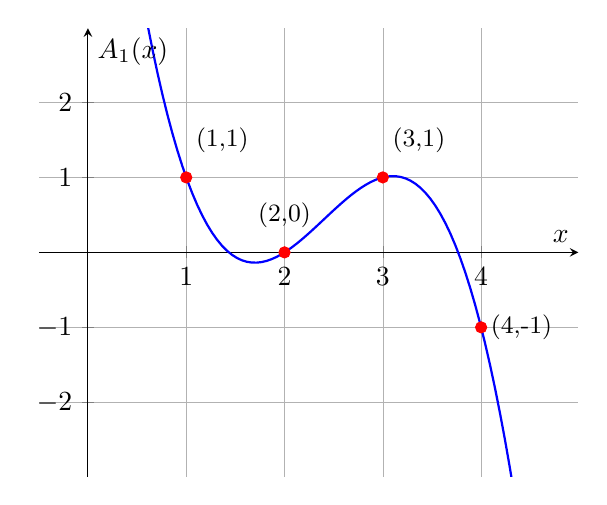
\begin{tikzpicture}
            \begin{axis}[
                axis lines = middle,
                xlabel = {$x$},
                ylabel = {$A_1(x)$},
                ymin = -2.99, ymax = 2.99,
                xmin = -0.5, xmax = 4.99,
                domain = 0:5,
                samples = 100,
                ytick = {-3,...,3},
                xtick = {0,1,...,5},
                grid = both, 
                grid style = {line width=.1pt, draw=gray!20},
                major grid style = {line width=.2pt, draw=gray!60}
            ]
            \addplot[
                color=blue,
                thick
            ]
            {-5/6*x^3 + 6*x^2 - 79/6*x + 9};
            \addplot[
                only marks,
                mark=*,
                color=red
            ]
            coordinates {(1,1) (2,0) (3,1) (4,-1)};
    
            \node at (axis cs:1,1.5) [anchor=west] {\small (1,1)};
            \node at (axis cs:2,0.2) [anchor=south] {\small (2,0)};
            \node at (axis cs:3,1.5) [anchor=west] {\small (3,1)};
            \node at (axis cs:4,-1) [anchor=west] {\small (4,-1)};
            
            \end{axis}
        \end{tikzpicture}

        \scriptsize\textbf{Illustration:} The Lagrange inteprolation polynomial for points $\{(1,1), (2,0), (3,1), (4,-1)\}$ visualized over $\mathbb{R}$.
    \end{center}
\end{example}

\begin{remark}
    The degree of the coefficient polynomials does not exceed $m - 1$, which follows from the Lagrange interpolation properties.
\end{remark}

\subsubsection{Putting All Together!}

Now, using coefficients encoded with polynomials, a constraint number $X \in \{1, \dots\ m\}$, from
a constraint system with a witness vector $\mathbf{w}$ can be built in the next way:
\begin{align*}
    (w_1A_1(X) + w_2A_2(X) + \dots + w_nA_n(X)) &\times (w_1B_1(X) + w_2B_2(X) + \dots + w_nB_n(X)) =\\ = (w_1C_1(X) + w_2C_2(X)& + \dots + w_nC_n(X))
\end{align*}

Or, written more concisely:
\begin{equation*}
    \left( \sum_{i = 1}^{n} w_iA_i(X) \right) \times \left( \sum_{i = 1}^{n} w_iB_i(X) \right) = \left( \sum_{i = 1}^{n} w_iC_i(X) \right)
\end{equation*}

\begin{remark}
    Hold on, but why does it hold? Let us substitute any $X=j$ into this equation:
    \begin{equation*}
        \left( \sum_{i = 1}^{n} w_iA_i(j) \right) \times \left( \sum_{i = 1}^{n} w_iB_i(j) \right) = \left( \sum_{i = 1}^{n} w_iC_i(j) \right) \; \forall j \in \{1,\dots,m\}
    \end{equation*}

    Recall that we interpolated polynomials to have $A_i(j) = a_{j,i}$. Therefore, the equation above can be reduced to:
    \begin{equation*}
        \left( \sum_{i = 1}^{n} w_ia_{j,i} \right) \times \left( \sum_{i = 1}^{n} w_ib_{j,i} \right) = \left( \sum_{i = 1}^{n} w_ic_{j,i} \right) \; \forall j \in \{1,\dots,m\}
    \end{equation*}

    But hold on again! Notice that $\sum_{i = 1}^{n} w_ia_{j,i} = \langle \mathbf{w}, \mathbf{a}_j \rangle$ and therefore we have:
    \begin{equation*}
        \langle \mathbf{w}, \mathbf{a}_j \rangle \times \langle \mathbf{w}, \mathbf{b}_j \rangle = \langle \mathbf{w}, \mathbf{c}_j \rangle \; \forall j \in \{1,\dots,m\},
    \end{equation*}
    
    so we ended up with the initial $m$ constraint equations!
\end{remark}

Now let us define polynomials $A(X)$, $B(X)$, $C(X)$ for easier notation: 
\begin{equation*}
    A(X) = \sum_{i = 1}^{n} w_iA_i(X), \quad B(X) = \sum_{i = 1}^{n} w_iB_i(X), \quad C(X) = \sum_{i = 1}^{n} w_iC_i(X)
\end{equation*}

Therefore, our constraint can be rewritten as $A + B = C$ --- much less scary-looking than what we have written before. OK, but what does it give us? 

Notice that if $A(X)+B(X)=C(X)$ for all $j \in \{1,\dots,m\}$ then polynomial, defined as $P(X) := A(X)+B(X)-C(X)$, has zeros at all elements from the set $\Omega = \{1,\dots,m\}$. Define the so-called \textbf{vanishing polynomial} on $\Omega$ as:
\begin{equation*}
    Z_{\Omega}(X) := \prod_{\omega \in \Omega} (X - \omega) = \prod_{i=1}^m (X - i)
\end{equation*} 

Now, if $P(X)$ vanishes on all points from $\Omega$, it means that $Z_{\Omega}$ must divide $P$, so $Z_{\Omega} \mid P$. But that means
that $P$ can be divided by $Z_{\Omega}$ without remainder! In other words, there exists some polynomial $H$ such that $P=Z_{\Omega}H$. All in all,
let us give the definition of a \textbf{Quadratic Arithmetic Program}.

\begin{definition}[Quadratic Arithmetic Program]
    Suppose that $m$ R1CS constraints with a witness of size $n$ are written in a form
    \begin{equation*}
        A\mathbf{w} \odot B\mathbf{w} = C\mathbf{w}, \; A,B,C \in \mathbb{F}^{m \times n}
    \end{equation*}

    Then, the \textbf{Quadratic Arithmetic Program} consists of $3n$ polynomials $A_1,\dots,A_n$, $B_1,\dots,B_n$, $C_1,\dots,C_n$ such that:
    \begin{equation*}
        A_j(i) = a_{i,j}, \; B_j(i) = b_{i,j}, \; C_j(i) = c_{i,j}, \; \forall i \in \{1,\dots,m\} \; \forall j \in \{1,\dots,n\}
    \end{equation*}

    Then, $\mathbf{w} \in \mathbb{F}^n$ is a valid assignment for the given QAP and \textbf{target polynomial} $Z_{\Omega}(X) = \prod_{i=1}^m (X-i)$ if and only if there exists such a polynomial $H(X)$ such that
    \begin{equation*}
        \left( \sum_{i = 1}^{n} w_iA_i(X) \right)\left( \sum_{i = 1}^{n} w_iB_i(X) \right) - \left( \sum_{i = 1}^{n} w_iC_i(X) \right) = Z_{\Omega}(X)H(X)
    \end{equation*}
\end{definition}

This was our final step in representing a high-level programming language to some math primitive.
We have managed to encode our computation to a single polynomial!

\subsubsection*{Remark on operations between polynomials}

\begin{remark}
    Some pretty obvious property should be noted. In the theorem ~\ref{thm:polynomials-degree-op}
    it was said about the degree of polynomials after their multiplication or addition, but what
    about their values?

    Let $p(x), q(x) \in \mathbb{F}[x]$ be two polynomials over a field $\mathbb{F}$. Define the 
    polynomial $r(x)$ as the sum of $p(x)$ and $q(x)$:
    \begin{equation*}
        r(x) = p(x) + q(x)
    \end{equation*}
    Then, for any point $x \in \mathbb{F}$, the value of $r(x)$ is equal to the sum of the
    values of $p(x)$ and $q(x)$ at that point. Therefore, the set of points corresponding to the 
    polynomial $r(x)$ is given by:
    \begin{equation*}
        \{(x, y) \in \mathbb{F} \times \mathbb{F} \mid x \in \mathbb{F}, \, y = p(x) + q(x) \}
    \end{equation*}

    The same is true for product.
\end{remark}

\begin{example}
    Consider two polynomials $p(x)$ and $q(x)$ defined over the real numbers $\mathbb{R}$:
    \begin{equation*}
        p(x) = -\frac{1}{2}x^2 + \frac{3}{2}x, \quad
        q(x) = \frac{1}{3}x^3 - 2x^2 + \frac{8}{3}x + 1.
    \end{equation*}
    The sets of points $\{(0, 0), (1, 1), (2, 1), (3, 0)\}$ and $\{(0, 1), (1, 2), (2, 1), (3, 0)\}$
    lie on the graphs of $p(x)$ and $q(x)$, respectively.\\
    
    The sum of these polynomials can be calculated as:
    \begin{align*}
        r(x) &= (-\frac{1}{2}x^2 + \frac{3}{2}x) + (\frac{1}{3}x^3 - 2x^2 + \frac{8}{3}x + 1) \\
             &= \frac{1}{3}x^3 - 2\frac{1}{2}x^2 + 4\frac{1}{6}x + 1
    \end{align*}
    The resulting polynomial $r(x)$ corresponds to the set of points $\{(0, 1), (1, 3), (2, 2), (3, 0)\}$.
    
    As you can see (Figure~\ref{fig:example-polynomial-addition}), the values at each point for the 
    corresponding $x$ are the sum of the initial polynomials' points.
\end{example}

\begin{figure}[H]
    \centering
    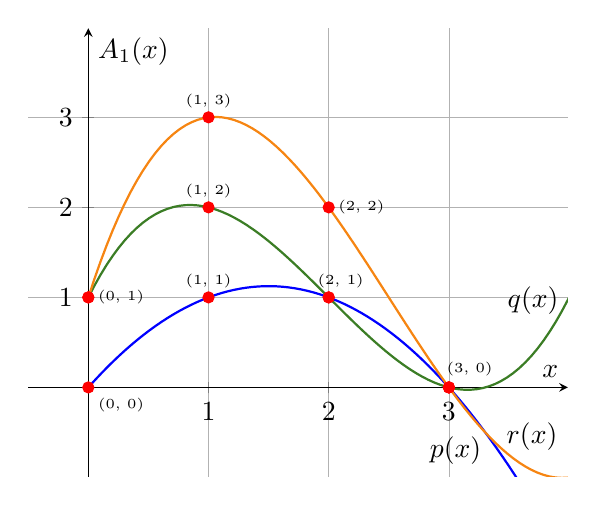
\begin{tikzpicture}
        \begin{axis}[
            axis lines = middle,
            xlabel = {$x$},
            ylabel = {$A_1(x)$},
            ymin = -0.99, ymax = 3.99,
            xmin = -0.5, xmax = 3.99,
            domain = 0:5,
            samples = 100,
            ytick = {-1,...,4},
            xtick = {0,1,...,4},
            grid = both,
            grid style = {line width=.1pt, draw=gray!20},
            major grid style = {line width=.2pt, draw=gray!60}
        ]

        % p(x)
        \addplot[
            color=blue,
            thick
        ]
        {3/2*x - 1/2*x^2};
        \addplot[
            only marks,
            mark=*,
            color=red
        ]
        coordinates {(0, 0) (1, 1) (2, 1) (3, 0)};
        \node at (axis cs:3.35,-0.7) [anchor=east] {\text{$p(x)$}};

        \node at (axis cs:0,-0.2) [anchor=west] {\tiny (0, 0)};
        \node at (axis cs:1,1) [anchor=south] {\tiny (1, 1)};
        \node at (axis cs:2.1,1) [anchor=south] {\tiny (2, 1)};
        \node at (axis cs:2.9,0.2) [anchor=west] {\tiny (3, 0)};

        % q(x)
        \addplot[
            color=OliveGreen,
            thick
        ]
        {1/3*x^3 - 2*x^2 + 8/3*x + 1};
        \addplot[
            only marks,
            mark=*,
            color=red
        ]
        coordinates {(0,1) (1,2) (2,1) (3, 0)};
        \node at (axis cs:3.7,0.7) [anchor=south] {\text{$q(x)$}};

        \node at (axis cs:0,1) [anchor=west] {\tiny (0, 1)};
        \node at (axis cs:1,2) [anchor=south] {\tiny (1, 2)};

        % r(x)
        \addplot[
            color=BurntOrange,
            thick
        ]
        {1/3*x^3 - 5/2*x^2 + 25/6*x + 1};
        \addplot[
            only marks,
            mark=*,
            color=red
        ]
        coordinates {(0,1) (1,3) (2,2) (3, 0)};
        \node at (axis cs:3.4,-0.55) [anchor=west] {\text{$r(x)$}};

        \node at (axis cs:1,3) [anchor=south] {\tiny (1, 3)};
        \node at (axis cs:2,2) [anchor=west] {\tiny (2, 2)};

        \end{axis}
    \end{tikzpicture}
    \caption{Addition of two polynomials}
    \label{fig:example-polynomial-addition}
\end{figure}

\subsection{Probabilistically Checkable Proofs}

Before going further we should get acquainted with one more concept from the computational 
complexity theory, that have an important application in zk-SNARK and provides the theoretical 
backbone. 

A Probabilistically Checkable Proof (PCP) is a type of proof system where the verifier can 
efficiently check the correctness of a proof by examining only a small, random portion of it, rather
than verifying it entirely. 
\begin{definition}
    A language $\mathcal{L} \subseteq \Sigma^*$ is in the class $PCP(r(n), q(n))$ if for a proof 
    $\pi \in \Sigma^*$ there exist a probabilistically polynomial time verifier $\mathcal{V}$ such
    that:
    \begin{itemize}
        \item The verifier receives an input $x \in \Sigma^n$ and access to a proof $\pi$, which it
            can query at any position.
        \item The verifier uses at most $r(n)$ random bits to decide which part of the proof to 
            query.
        \item The verifier queries at most $q(n)$ bits of the proof.
    \end{itemize}
    with following properties:
    \begin{itemize}
        \item \textbf{Completeness}: If $x \in \mathcal{L}$, there exist a proof 
            $\pi = \mathcal{P}(x)$ such that $\Pr{\mathcal{V}(x, \pi) = 1} = 1$
        \item \textbf{Soundness}: If $x \notin \mathcal{L}$, then for any proof 
            $\pi$, $\Pr{\mathcal{V}(x, \pi) = 1} = \mathsf{negl}(\lambda)$.
    \end{itemize}
\end{definition}
This allows a verification of huge statements with high confidence while using limited computational
resources.

\begin{theorem}{\textbf{PCP theorem (PCP characterization theorem)}\\}
    Any decision problem in $\mathsf{NP}$ has a PCP verifier that uses logarithmic randomness 
    $O(\log n)$ and a constant number of queries $O(1)$, independent of $n$.
    \begin{equation*}
        \mathsf{NP} = \mathsf{PCP}(O(\log n), O(1))
    \end{equation*}
\end{theorem}

\subsubsection{PCP application in QAP}

Constructing QAP we finished with a single polynomial $P(X)$:
\begin{equation*}
    P(X) = A(X)B(X) - C(X) = Z_{\Omega}(X)H(X)
\end{equation*}
We effectively managed to transform all the circuit's constraints, and computations in the short form.
It's still allows one to verify that each computational step is preserved by verifying the 
polynomial evaluation in specific points, instead of recomputing everything.

As it was said early, we perform all the computations in some finite field $\mathbb{F}_p$. The 
polynomials $A$, $B$ and $C$ are interpolated polynomials using $\left| w \right|$ points, so 
\begin{equation*}
    \deg(A) \le \left| w \right|, \quad 
    \deg(B) \le \left| w \right|, \quad 
    \deg(C) \le \left| w \right|
\end{equation*}
Thus, using properties of polynomials' degrees, we can estimate the degree of polynomial $P(X)$.
\begin{equation*}
    \deg(P) \leq \max(\deg(A) + \deg(B), \deg(C)) = \max(2 \left| w \right|, \left| w \right|) = 2 \left| w \right|
\end{equation*}

Now using \hyperref[lem:schwartz_zippel_lemma]{Schwartz-Zippel Lemma~\ref{lem:schwartz_zippel_lemma}},
we can state that if an adversary $\mathcal{A}$ doesn't know a valid witness $\mathbf{w}$ to 
resolves some circuit $\mathcal{C}$, they still can compute a polynomial $P(X)^{\prime}$ that 
satisfies a verifier $\mathcal{V}_{\mathcal{C}}$ with probability less then 
$\frac{2 \left| w \right|}{p}$.
\begin{equation*}
    \text{Pr}[ \mathcal{V}_{\mathcal{C}}(P(X)^{\prime}) = \mathsf{accept} \mid P(X)^{\prime} \xleftarrow{R} A] \leq \frac{2 \left| w \right|}{p}
\end{equation*}
This probability becomes negligible as $p$ grows large, giving us soundness. In the same time, the
verifier accepts the $P(X)$ generated using a valid witness with probability $1$ giving us the 
completeness, so, we can categorize QAP as PCP. 

We'll modify the form of our proof with the next modifications, but still preserve the PCP 
properties.

\end{document}